\section*{Questão 2}

\subsection*{Definição da Cadeia de Markov}

A cadeia de Markov para este problema é definida pelos seguintes elementos:

\begin{enumerate}
    \item \textbf{Estados}: Representados pela tupla $(c, s)$, onde:
    \begin{itemize}
        \item $c$ é o número de clientes no sistema (limitado entre 0 e 8).
        \item $s$ é o número de servidores disponíveis (limitado entre 1 e 3).
    \end{itemize}

    \item \textbf{Ações}: As ações disponíveis em cada estado são:
    \begin{itemize}
        \item $-1$: Remover um servidor.
        \item $0$: Manter o número atual de servidores.
        \item $+1$: Adicionar um servidor (respeitando os limites).
    \end{itemize}

    \item \textbf{Transições}: Determinadas pelas probabilidades de chegada de novos clientes no final de cada intervalo de tempo:
    \begin{itemize}
        \item $p_0 = 0.4$: Probabilidade de 0 clientes chegarem.
        \item $p_2 = 0.2$: Probabilidade de 2 clientes chegarem.
        \item $p_4 = 0.4$: Probabilidade de 4 clientes chegarem.
    \end{itemize}
    A transição entre estados considera:
    \begin{itemize}
        \item Atendimento: $\min(c, s)$ clientes são atendidos no início de cada intervalo.
        \item Clientes restantes: Permanecem no sistema para o próximo intervalo.
        \item Restrições: O número total de clientes no sistema é limitado a 8.
    \end{itemize}

    \item \textbf{Ordem dos eventos}: Para cada intervalo de tempo, a ordem dos eventos considerada é:
    \begin{enumerate}[label=\roman*.]
        \item Atendimento de clientes.
        \item Adição/remoção de servidores.
        \item Chegada de clientes.
    \end{enumerate}

    \item \textbf{Recompensas}: A recompensa para cada transição é composta por:
    \begin{itemize}
        \item Ganho por cliente atendido: $T \cdot \min(c, s)$, com $T = 10$.
        \item Custo por servidor: $-R_s \cdot s'$, com $R_s = 5$.
        \item Penalidade por fila: $-R_q$ se $c' > 4$, caso contrário $0$, com $R_q = 10$.
        \item Penalidade por ociosidade: $-R_0$ por servidor não utilizado, max($s' - c', 0$), com $R_0 = 2$.
    \end{itemize}
    Onde $c$ e $s$ são os valores de clientes e servidores no estado atual e $c'$ e $s'$ são os valores no próximo estado.
\end{enumerate}

\subsection*{Solução por \textit{Value Iteration}}

Foi implemmentado em Python uma função que calcula a política ótima para a cadeia de Markov descrita. O código fonte está disponível no repositório indicado no final deste relatório, na pasta \texttt{lista\_6}, arquivo \texttt{value\_itaration.py}. O código principal, onde são definidas as probabilidades de transição e as recompensas, está disponível no arquivo \texttt{main.py}. O código segue o seguinte fluxo:

\begin{enumerate}
    \item Inicializa \( V[s] = 0 \) para todos os estados \( s \).
    \item Iterativamente calcula os valores \( V[s] \) para cada estado, atualizando-os com base na equação de Bellman:
    \[
    V(s) = \max_a \sum_{s'} P(s' \mid s, a) \cdot \left( R(s, a, s') + \gamma \cdot V(s') \right).
    \]
    \item Em cada iteração, verifica a convergência comparando a maior mudança (\( \Delta \)) entre os valores antigos e novos. O loop termina quando \( \Delta < \theta \), o limiar definido.
    \item Após convergir, calcula a política ótima \( \pi^*(s) \) para cada estado, escolhendo a ação \( a \) que maximiza o valor esperado \( Q(s, a) \):
    \[
    \pi^*(s) = \arg\max_a \sum_{s'} P(s' \mid s, a) \cdot \left( R(s, a, s') + \gamma \cdot V(s') \right).
    \]
    \item Retorna a função de valor ótima \( V(s) \) e a política ótima \( \pi^*(s) \).
\end{enumerate}

Foi utilizado um fator de desconto $\gamma = 0.9$ e um limiar de convergência $\theta = 1e-6$. A função de valor ótima calculada e a política ótima derivada dela são apresentadas na figura \ref{fig:value_iteration_policy_and_values}.

\begin{figure}[H]
    \centering
    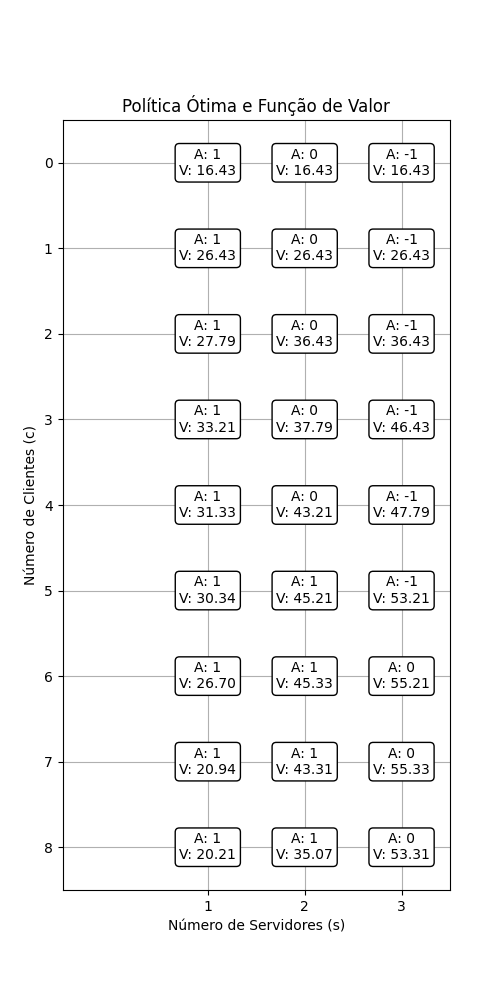
\includegraphics[width=0.5\textwidth]{fig/value_iteration_policy_and_values.png}
    \caption{Função de valor ótima e política ótima calculadas por \textit{Value Iteration}.}
    \label{fig:value_iteration_policy_and_values}
\end{figure}

O algoritmo convergiu em 2457 iterações. A variação de \( \Delta \) ao longo das iterações é apresentada na figura \ref{fig:value_iteration_delta}.

\begin{figure}[H]
    \centering
    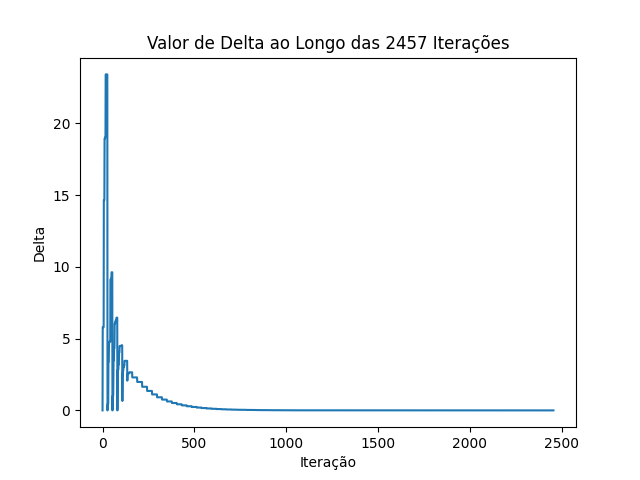
\includegraphics[width=0.5\textwidth]{fig/value_iteration_delta.png}
    \caption{Variação de \( \Delta \) ao longo das iterações de \textit{Value Iteration}.}
    \label{fig:value_iteration_delta}
\end{figure}
